\refstepcounter{Exercise}
\clearpage\subsection*{\theExercise CGIを使ってウェブページからLEDをつける}
\addtocounter{Exercise}{-1}\refstepcounter{Exercise}\label{E:CGI}

% \clearpage\subsection*{CGIを使ってウェブページからLEDをつける}

考え方

まずはラズパイにセンサーボードを取り付けましょう。今回はFaBoは使用しません。

ウェブサーバはウェブブラウザから要求を受けます。”ファイル名.hsp”ファイルへのアクセスをブラウザから行うとサーバはCGIプログラムをサーバ側で起動します。結果はHTMLとしてブラウザ(クライアント)へ返されます。

試しに、CGIプログラムを起動させてみましょう。例題のプログラムはLEDがすでに点灯していれば消灯、消灯してれば点灯するプログラムです。ウェブサーバがウェブブラウザから要求を受けて、CGIプログラムを起動するのでウェブサーバが起動している必要があります。まずはウェブサーバを起動させましょう。

ターミナルを開いて

cd {\textasciitilde}/07/www/

./webserver.py \ \ \ \ で起動できます。

%
%コマンド実行画面
%cd {\textasciitilde}/07/www/
%./webserver.py
%koyaman
%September 20, 2019 2:48 AM


次にウェブブラウザからウェブサーバへCGIの要求を出してみましょう。

ブラウザを開いて、

localhost:3000/cgi-bin/led.hsp

%
%ぶらうざで開いた画面
%koyaman
%September 20, 2019 2:49 AM


\centering
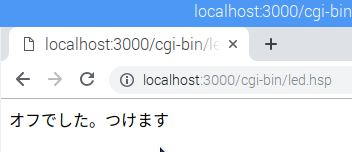
\includegraphics[width=0.7\textwidth]{text07-img/ome7-img051.png}
\flushleft

にアクセスをしてみましょう。アクセスをすると、プログラムが起動してLEDが点灯します。ブラウザのリロードボタンを押すと消灯します。

\centering
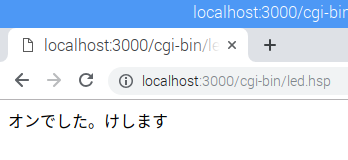
\includegraphics[width=0.7\textwidth]{text07-img/ome7-img052.png}
\flushleft

cgi-binディレクトリはCGIプログラムを入れるディレクトリです。{\textasciitilde}/07/wwwの下にあります。このディレクトリ内の

”ファイル名”.hsp

はCGIプログラムとして\ruby{扱}{あつ}われます。led.hspはCGIプログラムです。


\bigskip

\clearpage
プログラム解説


\begin{table}[htbp]
    \centering
    % \caption{文字タイプ表}
    \begin{tabular}{|l|}
        \hline
        
        1. \#include "hsp3cl.as"\\ 
        2. \#include "rpz-gpio-cl.as"\\
        3. \\
        4. mes "Content-type: text/html{\textbackslash}n"\\
        5. mes "{\textless}html{\textgreater}{\textless}head{\textgreater}{\textless}meta charset={\textbackslash}"utf-8{\textbackslash}"{\textgreater}{\textless}/head{\textgreater}{\textless}body{\textgreater}"\\
        6. \\
        7. ;現在のGPIO 17の\ruby{値}{あたい}を取得 1 == ON, 0 == OFF\\
        8. ;CGIからはcgpioinを使う(使い方はgpioinと同じ)\\
        9. prev\_led = cgpioin(17)\\
        10. \\
        11. if prev\_led = 0\{\\
        12. ;ついていなかった\\
        13. mes{\textquotedbl}{\textless}p{\textgreater}オフでした。つけます{\textless}/p{\textgreater}{\textquotedbl}\\
        14. next\_led = 1\\
        15. \}else\{\\
        16. ;\\
        17. mes{\textquotedbl}{\textless}p{\textgreater}オンでした。けします{\textless}/p{\textgreater}{\textquotedbl}\\
        18. next\_led = 0\\
        19. \}\\
        20. mes {\textquotedbl}{\textless}/body{\textgreater}{\textless}/html{\textgreater}{\textquotedbl}\\
        21. ;CGIからはcgpioを使う(使い方はgpioと同じ、0以外を書いた場合プログラムが\\
        22. ;\ruby{終了}{しゅうりょう}してもLEDは点灯し続ける)\\
        23. cgpio 17, next\_led\\
        24. end
        
        \\\hline
    \end{tabular}
\end{table}





第3回に使用した命令ではない命令が入っています。\\
詳細はP\pageref{P:gpio}に載っています。確認してください。
% 詳細はPに載っています。確認してください。

プログラム解説の4行目

mes {\textquotedbl}Content-type: text/html{\textbackslash}n{\textquotedbl}

はCGIプログラムがウェブサーバに結果を返すときに、結果がHTMLであることを伝えるために必要です。{\textbackslash}nは改行を意味します。本来は改行は2つ必要ですが、mes命令は自動で改行を入れてくれるので、{\textbackslash}nは1つで十分です。


\bigskip
\clearpage
4行目\ruby{以降}{いこう}のmes命令で出力するものは、HTMLの一部として扱われます。

\bigskip

6行目では、文字コードを設定しています。

\bigskip

9行目からLED点灯消灯のプログラムが始まります。

prev\_led = cgpioin(17)

では、GPIO17番の状態を調べています。LEDが点灯していれば1になり、消灯していれば0になります。


\bigskip


10〜17行目では、\ruby{条件}{じょうけん}判断のif文を使って読み取ったLEDの状態を判断します。消灯状態であれば、9行目で

mes
	{\textquotedbl}{\textless}p{\textgreater}オフでした。つけます{\textless}/p{\textgreater}{\textquotedbl}

pタグを使ってメッセージを表示します。

\bigskip

12行目で

next\_led = 1

としてLEDを点灯させるための値を用意します。

\bigskip

消灯以外の状態(つまり点灯状態)の場合は、13行目で

mes
	{\textquotedbl}{\textless}p{\textgreater}オンでした。けします{\textless}/p{\textgreater}{\textquotedbl}

pタグを使ってメッセージを表示します。

\bigskip

18行目で

next\_led = 0

としてLEDを消灯させるための値を用意します

\bigskip

20行目で実際に値をGPIO17へ書き込みます。

cgpio 17, next\_led




\bigskip

21行目の

end

でプログラムの終了をします。


\bigskip



第7回のCGIを使うプログラムでは、第3回の授業とはちがう命令を使います。\\
第3回の命令でCGIを使おうとすると、上手く動かなくなってしまうからです。\\
下の表にそれぞれの命令をまとめておきます。\\

\clearpage



\begin{table}[htbp]
    \centering
    % \caption{文字タイプ表}
    \begin{tabular}{|l|l|l|}
        \hline
        第3回に使った命令名 & CGIを使うときの命令名 & 効果
		\\\hline

        \begin{tabular}{l}
            \#include “rpz-gpio.as”
        \end{tabular}
        &
        \begin{tabular}{l}
            \#include “rpz-gpio-cl.as”
        \end{tabular}
        &
        \begin{tabular}{l}
            プログラムのはじめに書くことでLED\\
		    の点灯や消灯の命令が使えるようにな\\
            ります。
        \end{tabular}
        \\\hline

        \begin{tabular}{l}
            onoff\ = \ gpioin(17)
        \end{tabular}
        &
        \begin{tabular}{l}
            onoff\ = \ cgpioin(17)
        \end{tabular}
        &
        \begin{tabular}{l}
            17番のGPIOのLEDが点灯していれ\\
            ば変数onoffに1が、消灯していれば変\\
            数onoffに0が入ります。17をほかの番\\
            号に変えることで、ほかのLEDの状態\\
            を確認できます。
        \end{tabular}
        \\\hline

        \begin{tabular}{l}
            gpio \ 18,\ 1
        \end{tabular}
        &
        \begin{tabular}{l}
            cgpioin \ 18,\ 1
        \end{tabular}
        &
        \begin{tabular}{l}
            18番のGPIOのLEDを点灯します。1\\
            を0にすると消灯になります。18をほ\\
            かの番号に変えることで、ほかのLED\\
            を点灯、消灯できます。
        \end{tabular}
        \\\hline
        
    \end{tabular}
    \end{table}



\bigskip


\bigskip
\refstepcounter{Question}\theQuestion

% 問題7-10  
{\bfseries
	友達のLEDをCGIで点灯させてみよう。}

{\bfseries

	点灯、消灯時のウェブページに表示されるメッセージを\ruby{変更}{へんこう}してみよう。}

{\bfseries
	他の色のLEDも点灯、消灯できるようにしよう。}

{\bfseries
	Faboのセンサ(LED,
	\ruby{振動子}{しんどうし}などのデジタルセンサ)を接続してCGIから動かせるようにしてみよう。}


\bigskip